\section{Software Usage}

This section explains the usage of the Quartus Software as well as the usage of the two provided template projects.

\subsection{Quartus How-To}

The Quartus splash screen offers two frequently needed options: \textit{New Project Wizard} and \textit{Open Project}. For the template Projects the \textit{Open Project} option opens a file manager that is used to open the project file. The Project file is located in the directory of the project and has the file extension \textit{.qpf}.

\subsubsection{Project Navigator}

The left side of the Quartus window shows the \textit{Project Navigator} which is used to navigate through the project. In its default state it shows a hierarchy of the project files but it can be switched to a file view as shown in \cref{fig:quartus_project_navigator}.

\begin{figure}[h!]
	\centering
	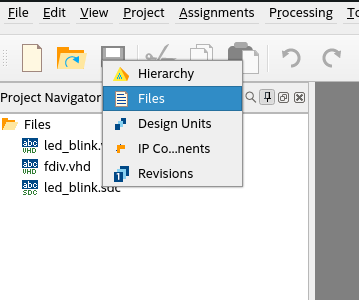
\includegraphics[width=0.5\textwidth]{fig/quartus_project_navigator.png}
	\caption{The Quartus project navigator allows to navigate through the project files.}
	\label{fig:quartus_project_navigator}
\end{figure}

The files can be edited by double-clicking on them in the project navigator.

\subsubsection{Synthesis}

To synthesize a design the Quartus Software has two methods to start the synthesis process. The first method is to click on the \textit{Start Compilation} button in the toolbar. The second method is to double click on the \textit{Compile Design} entry in the \textit{Tasks} window. The \textit{Tasks} window is located in the bottom left corner of the Quartus window. Both options are highlighted in \cref{fig:quartus_start_synthesis}. The synthesis process can take a few minutes depending on the complexity of the design. Any errors that occur during the synthesis process are shown in the \textit{Messages} window which is located in the bottom of the Quartus window.

\begin{figure}[h!]
	\centering
	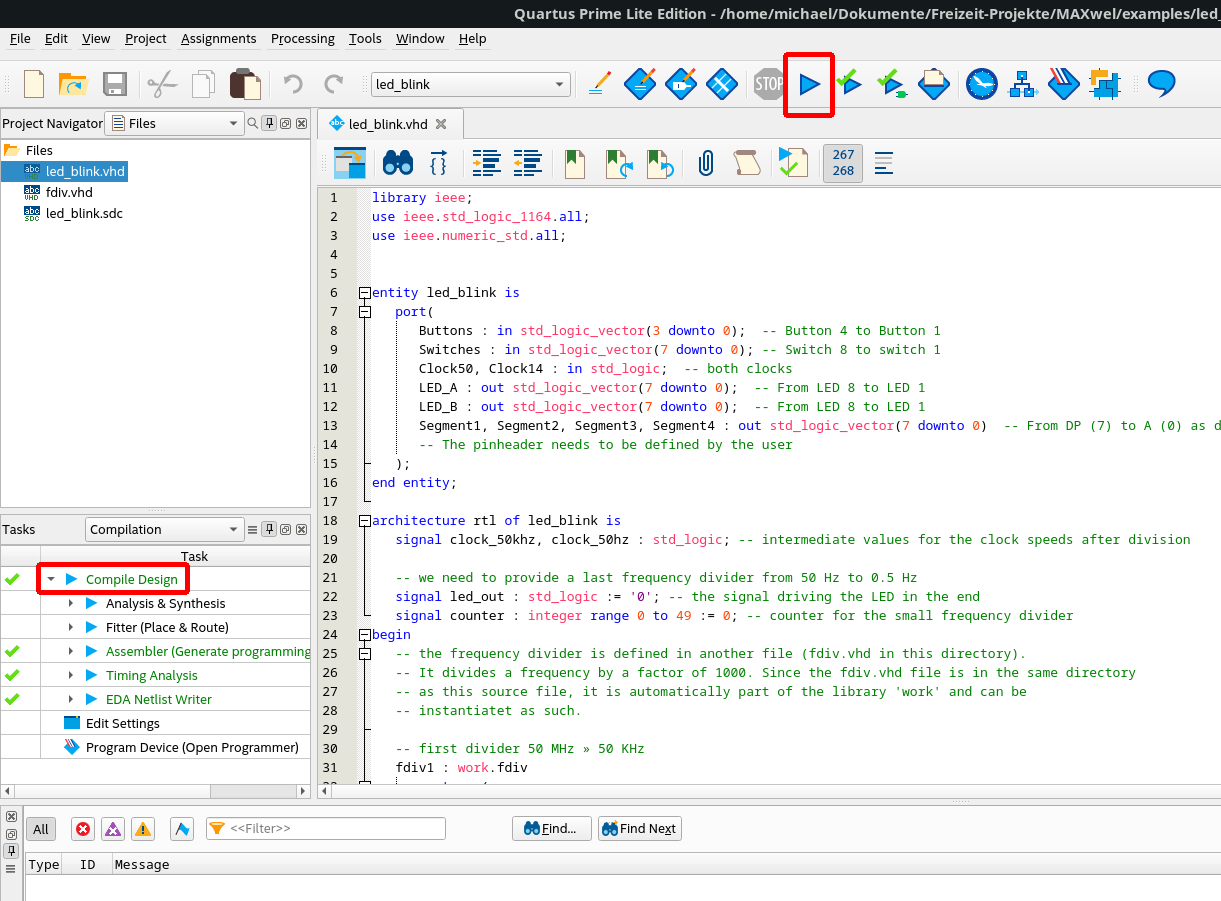
\includegraphics[width=0.9\textwidth]{fig/quartus_start_synthesis.png}
	\caption{There are two ways to start a synthesis}
	\label{fig:quartus_start_synthesis}
\end{figure}

\subsubsection{Programming the FPGA}

The synthesized design can be uploaded using the \textit{Programmer} tool. The programmer tool can be opened by clicking on the \textit{Programmer} button in the toolbar or double clicking the \textit{Program Device} entry in the \textit{Tasks} window. Both options are highlighted in \cref{fig:quartus_start_programmer}.

\begin{figure}[h!]
	\centering
	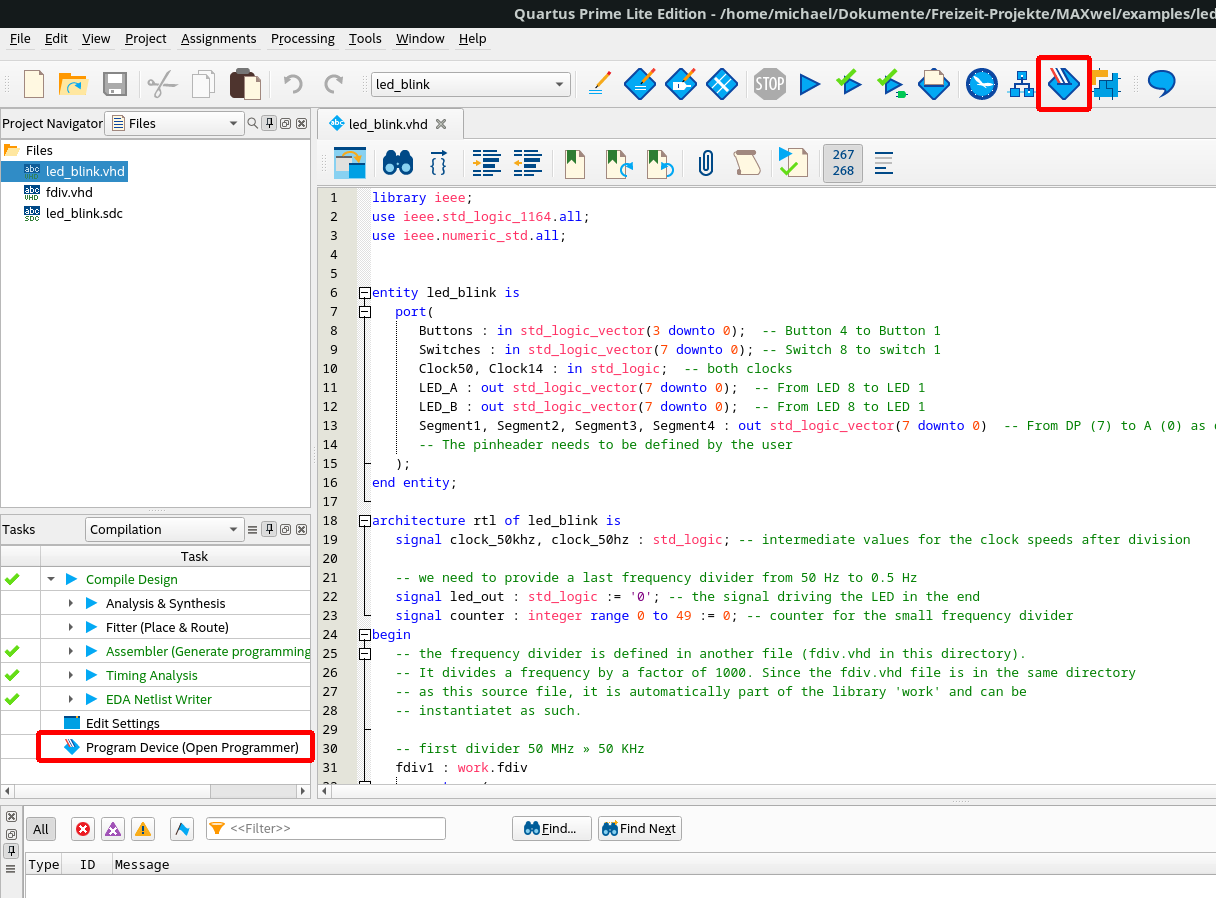
\includegraphics[width=0.9\textwidth]{fig/quartus_start_programming.png}
	\caption{Possibilities to open the programmer tool.}
	\label{fig:quartus_start_programmer}
\end{figure}

The dialog window of the programmer tool is shown in \cref{fig:quartus_programmer}. There, the \textit{Hardware Setup} can be configured to select a programmer device. Afterwards, the checkbox of the "CFM" file (the synthesis result) has to be checked for the option \textit{Program/Configure}. By clicking on the \textit{Start} button the design is uploaded to the FPGA. The important buttons are highlighted in \cref{fig:quartus_programmer}.

\begin{figure}[h!]
	\centering
	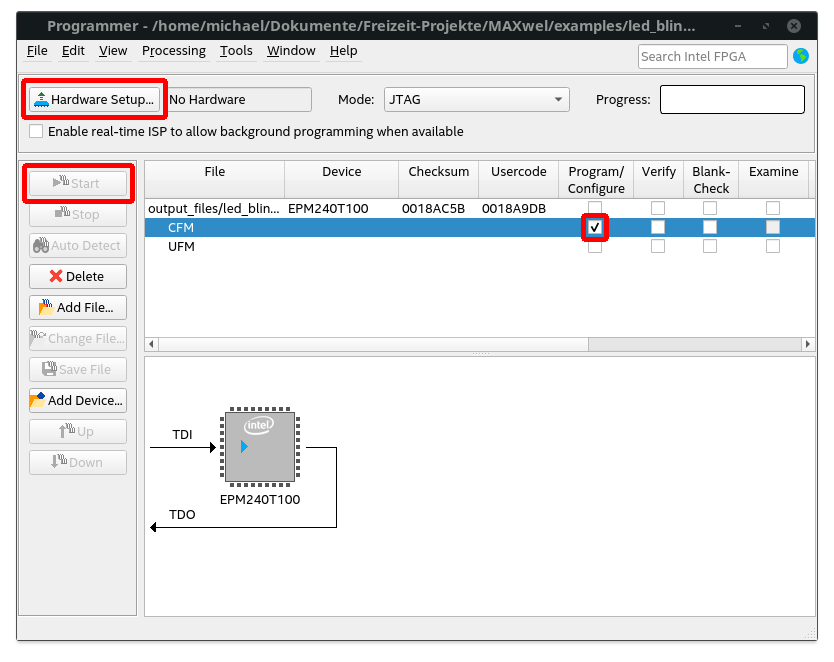
\includegraphics[width=0.9\textwidth]{fig/quartus_programmer.png}
	\caption{Important sections of the Programmer dialog}
	\label{fig:quartus_programmer}
\end{figure}

\subsection{Template Projects}

The template projects have been created using the \textit{New Project Wizard}. During this setup, the target device needs to be specified. For the MAXwel board it is the \textit{EPM250T100C5} Chip. Afterwards an empty project should be available. The Input / Output pins of the FPGA can be configured by selecting the \textit{Pin Planner} in the \textit{Assignments} menu. This allows to assign the pins to the desired signals, which is already done in the template projects. It is important that the pins assigned to the Switches and Buttons have the value in the \textit{I/O Standard} column set to \textit{3.3V Schmitt Trigger Input} whereas the other pins can stay at the default value \textit{3.3V LVCMOS}. The informations specified in the pin planner are also located in the \textit{.qsf} file of the project.
